% When making labels follow the Labels and Cross-referencing guide
%
% http://en.wikibooks.org/wiki/LaTeX/Labels_and_Cross-referencing#Introduction
\bibliography{../References/refer}

\section{Abstract}
    The quicksort is a thoroughly studied sorting algorithm and is commonly among the first efficient sorts learned by students of computer science. Many variants of the quicksort have been proposed, from the classic quicksort introduced by Tony Hoare in 1961 \cite{Hoare01011962} to Yaroslavskiy’s dual pivot quicksort introduced in 2009 and used by the Java 7 Standard Library \cite{kushagra2013multi}. Since Hoare’s first proposal, much research has gone into attempting to minimize the total number of swaps done by the sort, the total number of comparisons done by the sort and minimizing the worst case runtime. We aim to experimentally validate the swap and comparison count of several variants of the quicksort and compare the runtimes and various optimizations. Our results SUMMARIZE THE RESULTS

\section{Introduction}
    Sorting is a fundamental concept of computer science wherein a totally ordered multiset is modified such that the elements of the multiset are rearranged (permuted) in either non-decreasing or non-increasing order. A broad range of applications benefit from sorting such as organizing an MP3 library by song title to quickly identifying duplicates in a list to more advanced applications such as load balancing, data compression and computer graphics \cite{sortingSlides}. It is well known that all comparison based sorting algorithms are lower bound by $\Omega(n log n)$ comparisons \cite{Cormen:2001:IA:580470} and quicksort is no exception to this rule. Interestingly, there are non-comparison based sorts such as the counting sort and the radix sort which take advantage of certain properties of the data set and get around the lower bound of comparison base sorts. A summary of space and time complexities can be found in Table \ref{tab:spaceAndTime}.
    
    \begin{table}
        \begin{center}
            \begin{tabular}{|l|l|l|l|}
                    \hline
                    Sort Method &   Space       &   Average Case Time   &   Worst Case Time     \\ \hline \hline
                    Selection   &   $O(1)$      &   $O(n^2)$            &   $O(n^2)$            \\ \hline
                    Insertion   &   $O(1)$      &   $O(n^2)$            &   $O(n^2)$            \\ \hline
                    Merge       &   $O(n)$      &   $O(n\log(n))$       &   $O(n\log(n))$       \\ \hline
                    Quicksort   &   $O(1)$      &   $O(n\log(n))$       &   $O(n^2)$            \\ \hline
                    Radix       &   $O(n)$      &   $O(n*k)$            &   $O(n*k)$            \\ \hline
                    Counting    &   $O(m)$      &   $O(n+m)$            &   $O(n+m)$            \\ \hline
                \end{tabular}
                \caption{Summary of space and time complexities of various sorts where $n$ represents the number of elements, $k$ represents the number of digits in the largest value and $m$ represents the maximum value to be sorted. }
                \label{tab:spaceAndTime}
        \end{center}
    \end{table}

    The quicksort was first introduced by Tony Hoare in \cite{Hoare01011962} and was quickly adopted by the field as a standard sorting algorithm alongside the mergesort \cite{Knuth:1998:ACP:280635} and several other sorting algorithms. Quicksorts simplicity, high average case performance, poor worst case performance and low use of additional memory has made it one of the most highly studied ``efficient'' sorting algorithms. van Emden \cite{van1970increasing} proposed an optimization to the quicksort in 1970 which resulted in a 15\% improvement on the efficiency of the quicksort. In 1971 Hoare and Foley \cite{foley1971proof} provided a formal proof of other correctness of the quicksort. In 1977, Sedgewick did a thorough analysis of quicksort \cite{sedgewick1977analysis} and then in 1978 Sedgewick again published a paper on the quicksort exploring various implementations and proposing several optimizations \cite{sedgewick1978implementing}. The academic interest in the quicksort has not slowed since the late 1970s; papers regarding the quicksort continue to be published for adapting the quicksort to GPUs \cite{cederman2009gpu}, providing optimal pivot selection \cite{martinez2001optimal} and using more than one pivot \cite{edmondson2005m}. 

    In this paper we explore, compare and contrast the classic implementation of the quicksort against various multipivot quicksort implementations and their respective optimizations. We are particularly interested in comparing the classic quicksort against the standard dual pivot quicksort, Yaroslavskiy's dual pivot quicksort\cite{yaroslavskiy2009dual}, Aum\"{u}ller and Dietzfelbinger's optimized dual-pivot quicksort \cite{Aumuller:2013:OPD:2525857.2525862}, Edmonson's M-Pivot quicksort \cite{edmondson2005m} and the three pivot quicksort introduced by Kushagra et al \cite{kushagra2013multi}. We will first introduce the various quicksorts by providing a brief overview of their behaviour, implementation and potential optimizations. Next we will discuss the experiments and provide their results. Following this we provide an analysis, discuss future work and conclude the paper. 

\section{Quicksort}
	The following descriptions will assume that the algorithms are being used to sort a list $A$ in non-decreasing order where $n$ denotes the number of elements in $A$. Additionally, all algorithms are assumed to perform the sort in place. 

	\subsection{Classic Quicksort}
		\label{subsec:ClassicQSortIntro}
        The classic quicksort, first introduced by Hoare \cite{Hoare01011962} in 1962 is a recursive sorting algorithm which falls into the category of divide and conquer algorithms. All of following variations of the quicksort have these qualities as well. Quicksort can be summarized as follows:
        \begin{enumerate}
			\item Select a pivot in the current range of elements to be sorted.
			\item Partition the list such that all elements less than the pivot appear to the left of the pivot while all elements greater than or equal to the pivot appear to the right of the pivot.
			\item Recursively call quicksort on the left and right halves of the currently partitioned range.
        \end{enumerate}

        This na\"{i}ve implementation does not handle it's worst case gracefully. The classic quicksort degrades to a time complexity of $\BigOh{n^2}$ when the data being processed is in nearly sorted or already sorted order. Due to the simplicity of this implementation there are some minor changes which can be made to speed up the average case and aid the worst case runtimes. It was shown by Cook and Kim \cite{cook1980best} that insertion sorts are the fastest sort for small lists and nearly sorted lists. This optimization does not make the quicksort asymptotically faster than it's na\"{i} variation in either the average or worst case but does provide a meaningful speedup. Cook and Kim also showed that a hybrid of insertion sort and quicksort outperforms either of the sorts used individually. A perfectly selected pivot (the median of the range) would ensure that the worst case space complexity is bound by $\BigOh{n\log(n)}$. Perfect pivot selection cannot be achieved with an increase in time complexity; however, selecting pivot to be the median of first, middle and last elements is a good enough estimation of the true median of the range \cite{sedgewick1978implementing}.


	\subsection{Dual Pivot Quicksort}
		\label{subsec:DualPivotQSortIntro}

        The dual pivot quicksort is a variation of the classic quicksort which uses two pivots as opposed to one. 
	
	\subsection{Yaroslavskiy Quicksort}    
        \label{subsec:YaroslavskiyQSortIntro}
		Yaroslavskiy wished to make further optimizations to the dual pivot quicksort. Yaroslavskiy partion algorithm, even though based of the same abstract algorithmic idea produces different results\cite{Wild:2012:ACA:2404160.2404231}. The algorithm uses a five element sorting network to pick the two best elements. Then partitions intelegently by picking the "beter" comparison first\cite{Wild:2012:ACA:2404160.2404231}.
		
    \subsection{Optimal Dual Pivot Quicksort}
		\label{subsec:OptimalDualPivotQSortIntro}
		To further build on on the dual pivot quicksort and the Yaroslavskiy quicksort\cite{Aumuller:2013:OPD:2525857.2525862}. The pivots are selected as one sees fit, but when partitioning we keep track of how many elements that have been placed into the small list and the big list, denote these $N_s$ and $N_l$ respectivly. This idea is very similar to Yaroslavskiy's quicksort algorihm. Note that there are three category of elements in the dual pivot quicksort. When $N_s > N_l$ during the partition process, you first compare the the small pivot, otherwise compare to the large pivot. Although this is a simple optimization, the paper expends most of it's effort in proving that is the case\cite{Aumuller:2013:OPD:2525857.2525862}. With this small optimization the number of comparisions is drasically decreases relative to most quicksort implementations.
		
	\subsection{Three Pivot Quicksort}	
		\label{subsec:ThreePivotQSortIntro}	
		With the optimizations introduced from the Yaroslavskiy's quicksort algorithm and the optimal dual pivot quicksort algorithm, work has been done to see if similar benifites can achived from three pivots. The three pivot quicksort algorithm as described by Kushagra-Ortiz-Qiau-Munro. They present an algorithm that intelegently partitions the list into four segments \cite{kushagra2013multi}. When selecting pivots we have decided that we select pivots five points in the list that are evenly spaced, use insertion sort on these elemets, then pick the second and fourth element.
		
	\subsection{M Pivot Sort}	
		\label{subsec:MPivotQSortIntro}
		
		In 2007 a patent was published for the $M$-pivot quicksort \cite{edmondson2007multiple}. The algorithm uses ideas from probability and is concidered to be a natural extention to the dual pivot quicksort and the three pivot quicksort. The concept hopes to take the best parts of quicksort and also deal with problems that quicksort faces. $M$-pivot sort select $M$ pairs of elements positioned linearly throught the list (or sub-list).  Thus $2M$ elements have been selected as potential pivots. The entries are moved to the end of the list then sorted with an algorithm that works well on small list sizes (like insertion sort). This is shown in Figure \ref{fig:MPivotSelecton}.
		\begin{figure}[ht!]
			\begin{center}
				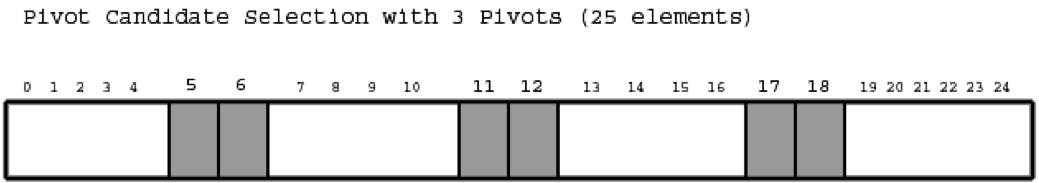
\includegraphics[width=70mm]{MPivotSelectCanadates.png}
				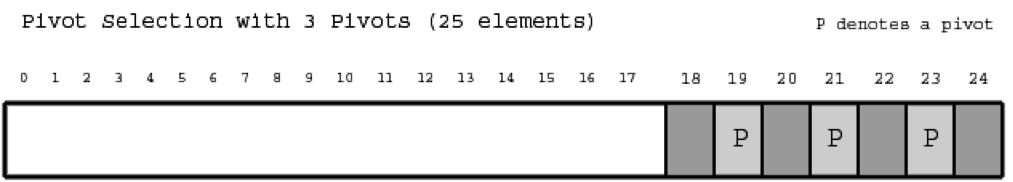
\includegraphics[width=70mm]{MPivotSelection.png}
				\caption{Diagram of how pivot selection is done in the $M$-pivot sort algorithm.}
				\label{fig:MPivotSelecton}
			\end{center}
		\end{figure}
		%******************************************************
		% Talk about M-Pivot Partitioning
		%******************************************************
		After the $M$ pivots are selected then we partition as demonstrated in Figure \ref{fig:MPivotPartition}. For each pivot we cycle through the array and group element together less than the current pivot. Then we recurse in the into that sublist.
		\begin{figure}[ht!]
			\begin{center}
				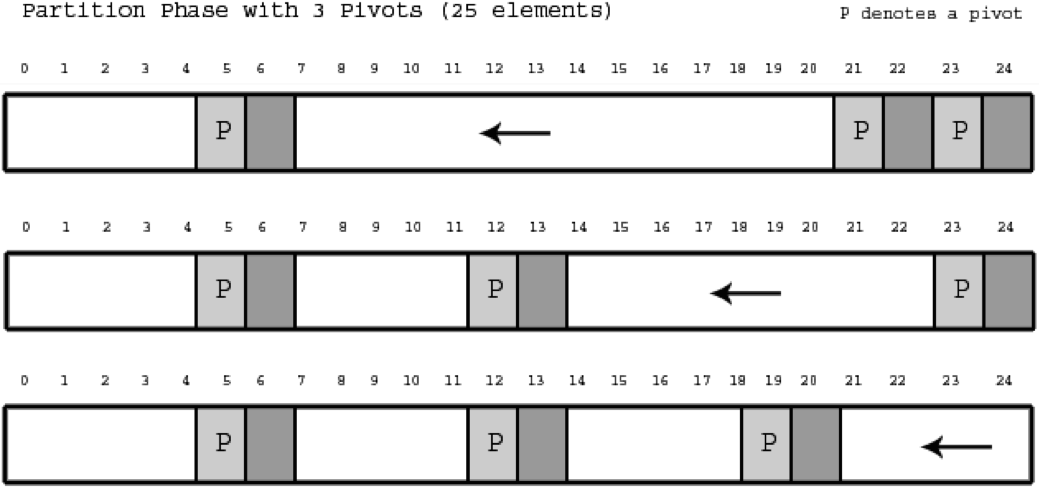
\includegraphics[width=70mm]{MPivotPartiton.png}
				\caption{How partitioning is done in the $M$-pivot sort algorithm.}
				\label{fig:MPivotPartition}
			\end{center}
		\end{figure}
		There are a few optimizations that can be made before starting any part of the algorithm (within the stack frame)\cite{edmondson2007multiple}. Before the call to the $M$-pivot sort, we can enforce that the min-heap property is applied. One call to the min-heapify function would only add $\BigOh{n}$ time and would not change the asympotic runtime of the algorithm.
		
		There are two more optimizations that could be applied. If one or more pivots end up having the same value then a different pivot is selected\cite{edmondson2007multiple}. The other optimization that could be made is that if all the pivots are found to be close to one side of the list, then the number of pivots is changed\ref{edmondson2007multiple}. The previously two stated optimizations not further studied in this paper.

	\subsection{Summary}
		%***************************************************************************************************
		% Tables will automatically move around when more text is added.
		% LaTeX is trying to place the tables [an soon enough figures too when I add them]
		% into "nice" places so that text is the least "messed" up.
		% So don't worry that the tables are all over the place [which includes before the introduction]
		% Even though the code for the tables are clearly after it.
		%***************************************************************************************************
		\begin{table}
			\begin{center}
				\begin{tabular}{|r|l|}
					\hline
					Sort Method        &   Comparisons                          \\ \hline \hline
					Classic            &   $2n \log n - 1.51n  + O(\log(n))$    \\ \hline
					Dual Pivot         &   $2.13n \log n - 2.57n + O(\log(n))$  \\ \hline
					Optimal Dual Pivot &   $1.8n \log n + O(n)$                 \\ \hline
					Three Pivot        &   $1.846n \log n + O(n)$               \\ \hline
					Yaroslavskiy       &   $1.9n \log n - 2.46n + O(\log(n))$   \\ \hline
					M Pivot            &   $O(n \log n)$                        \\ \hline
				\end{tabular}
				\caption{Summary table of theoretical comparisons.\ref{edmondson2007multiple}\cite{kushagra2013multi}\cite{Aumuller:2013:OPD:2525857.2525862}\cite{Wild:2012:ACA:2404160.2404231}}
				\label{tab:CompSummary}
			\end{center}
		\end{table}

		\begin{table}
			\begin{center}
				\begin{tabular}{|r|l|}
					\hline
					Sort Method         &     Swaps \\ \hline \hline
					Classic             &  $0.33n \log n - 0.58n + O(\log(n))$ \\ \hline
					Dual Pivot          &  $0.8n \log n -0.3n + O(\log(n))$    \\ \hline
					Optimal Dual Pivot  &  $0.33n \log n + O(n)$               \\ \hline
					Three Pivot         &  $0.615n \log n + O(n)$              \\ \hline
					Yaroslavskiy        &  $0.6n \log n + 0.08n + O(\log(n))$  \\ \hline
					M Pivot             &  $O(n \log n)$                       \\ \hline
				\end{tabular}
				\caption{Summary table of theoretical swaps.\ref{edmondson2007multiple}\cite{kushagra2013multi}\cite{Aumuller:2013:OPD:2525857.2525862}\cite{Wild:2012:ACA:2404160.2404231}}
				\label{tab:SwapSummary}
			\end{center}
		\end{table}